\documentclass[UTF8,zihao=-4,fontset=fandol,a4paper]{ctexart}
\usepackage[a4paper,left=23mm,right=23mm,top=21mm,bottom=22mm]{geometry}
\usepackage{amsmath,amssymb,booktabs,tabularx,array,graphicx,caption,multicol,placeins}
\usepackage[backend=biber,style=gb7714-2025,sorting=none,doi=true]{biblatex}
\addbibresource{literature.bib}
\addbibresource{methods.bib}
\usepackage[unicode,hidelinks,bookmarksnumbered]{hyperref}
\urlstyle{same}
\graphicspath{{figures/}{../图表/figures/}}

\newcommand{\papertitle}{央行货币政策执行报告文本情绪与 A 股行业收益}
\newcommand{\papersubtitle}{度量、预测与异质性检验}
\hypersetup{pdftitle={\papertitle{}：\papersubtitle},pdfauthor={王文楠，李享晨，何卓宁},pdfsubject={智能体科研创新挑战赛论文初稿}}
\ctexset{
  section={name={第,章},number=\chinese{section},format=\Large\bfseries,beforeskip=1.25ex,afterskip=0.85ex},
  subsection={number=\arabic{section}.\arabic{subsection},format=\large\bfseries,beforeskip=1.05ex,afterskip=0.45ex},
  subsubsection={number=\arabic{section}.\arabic{subsection}.\arabic{subsubsection},format=\normalsize\bfseries,beforeskip=0.8ex,afterskip=0.3ex}
}
\captionsetup{font=small,labelfont=bf,labelsep=quad,skip=4pt}
\captionsetup[table]{position=above}
\setlength{\textfloatsep}{10pt plus 2pt minus 2pt}
\setlength{\floatsep}{9pt plus 2pt minus 2pt}
\setlength{\intextsep}{8pt plus 2pt minus 2pt}
\setlength{\emergencystretch}{2em}
\setcounter{topnumber}{4}
\setcounter{bottomnumber}{2}
\setcounter{totalnumber}{5}
\setcounter{tocdepth}{1}
\setcounter{secnumdepth}{3}
\renewcommand{\topfraction}{0.84}
\renewcommand{\bottomfraction}{0.74}
\renewcommand{\textfraction}{0.13}
\raggedbottom
\newcommand{\paperfigure}[4]{%
  \begin{figure}[!htbp]
    \centering
    \includegraphics[width=#4\linewidth,height=0.42\textheight,keepaspectratio]{#1}
    \caption{#2}\label{#3}
  \end{figure}}

\begin{document}
\hypersetup{pageanchor=false}
\begin{titlepage}
  \thispagestyle{empty}
  \centering
  \vspace*{22mm}
  {\zihao{3}\bfseries 山东财经大学\par}
  \vspace{5mm}
  {\zihao{4} 首届智能体科研创新挑战赛\par}
  {\large Agentic Research Challenge 2026\par}
  \vspace{12mm}
  {\small 经济金融与社会科学智能分析赛道\quad 本科生组\par}
  \vspace{18mm}
  \rule{0.90\textwidth}{0.6pt}\par
  \vspace{8mm}
  {\zihao{1}\bfseries 央行货币政策执行报告\par}
  \vspace{3mm}
  {\zihao{1}\bfseries 文本情绪与 A 股行业收益\par}
  \vspace{5mm}
  {\zihao{3}\papersubtitle\par}
  \vspace{7mm}
  \rule{0.90\textwidth}{0.6pt}\par
  \vspace{14mm}
  {\zihao{-4}
  \renewcommand{\arraystretch}{1.36}
  \begin{tabular}{@{}r@{\hspace{1.4em}}l@{}}
    队名 & 秋珊百绘 \\
    作者 & 王文楠（金融学院）\\
         & 李享晨（金融学院）\\
         & 何卓宁（创新创业教育学院）\\
    指导教师 & 许中国 \\
  \end{tabular}\par}
  \vfill
  {\small 论文初稿 v1.0\quad 2026 年 11 月 20 日\par}
  \vspace{9mm}
\end{titlepage}

\pagenumbering{Roman}
\hypersetup{pageanchor=true}
\section*{摘要}
\addcontentsline{toc}{section}{摘要}
本文使用 2001 年第一季度至 2026 年第三季度的 103 期《中国货币政策执行报告》，结合申万一级行业指数，比较词典法与大语言模型评分，并采用事件研究、逐季横截面预测、行业交互模型和组合回测。主词典与归档抽检分值的相关为 0.695，但评分来源和独立性尚待核验。短窗关联在多重检验校正后缺乏统计支持。原收益窗口下，文本模型与无文本基准在共同测试样本上的样本外 $R^2$ 分别为 $-0.60$ 和 $-0.56$。改用发布后首个完整季度收益，并仅以预测时已实现收益训练后，文本模型仍弱于基准。行业特征难以解释敏感度差异，大语言模型的排序表现也未转化为稳定增量。现有证据不足以支持将报告情绪单独用于行业配置。

\noindent\textbf{关键词：} 货币政策执行报告；文本情绪；行业收益；样本外预测；大语言模型；事件研究

\vspace{0.9em}
\begin{center}
  {\large\bfseries Textual Sentiment in China's Monetary Policy Reports and A-Share Industry Returns}\par
  \vspace{0.2em}
  {\normalsize Measurement, Prediction, and Industry Heterogeneity}
\end{center}
\noindent\textbf{Abstract.}
Can the tone of the People's Bank of China's Monetary Policy Reports improve forecasts of A-share industry returns? We compare dictionary and large language model scores for 103 quarterly reports and evaluate them using event studies, sequential cross-sectional forecasts, industry regressions, and long-short portfolios. The main dictionary score correlates with archived reference scores ($r=0.695$), whose provenance and independence remain unverified. Short-window associations do not survive multiple-testing corrections. The text-augmented model underperforms the text-free baseline in out-of-sample $R^2$ on a common sample. The result holds when forecast targets are restricted to the first full quarter after publication and fitting uses only returns realized before the forecast date. Industry characteristics do not reliably explain differences in sensitivity, and the large language model yields no consistent improvement over the dictionary. The evidence does not support using report tone as a standalone industry allocation signal.

\noindent\textbf{Keywords:} monetary policy reports, textual sentiment, industry returns, out-of-sample prediction, large language models, event study

\clearpage
\tableofcontents
\vspace{1em}
\begingroup
\small
\setlength{\columnsep}{1.7em}
\begin{multicols}{2}
  \listoffigures
  \listoftables
\end{multicols}
\endgroup
\clearpage
\pagenumbering{arabic}

\section{绪论}
\label{sec:introduction}

\subsection{研究背景与意义}

货币政策通过政策工具的实际操作改变金融条件，也通过公开沟通改变市场对未来政策路径和经济前景的判断。中国人民银行按季发布的《中国货币政策执行报告》（下称 MPR）同时记录经济运行、政策执行和下一阶段政策思路，为在统一发布节奏下研究书面沟通提供了文本样本。报告中较积极的措辞可能伴随较好的增长预期。市场也可能据此修正对进一步宽松的预期。前者主要涉及预期现金流，后者可能通过贴现率发挥作用，两种机制对价格的作用方向未必一致。

行业层面的问题是，市场收到同一份报告后，各行业的相对收益能否呈现稳定的排序。即使股票市场整体在发布后上涨，各行业若以近似幅度反应，市场平均收益的变化也难以转化为行业配置价值。相反，行业的融资结构、现金流久期和政策暴露不同，可能使相同信息在行业间产生差异。因而，检验行业收益的增量可预测性，需要显式区分发布附近的异常收益、跨行业的相对收益，以及投资者在信号可得之后能够实现的收益。

\subsection{文献综述}

\subsubsection{MPR 文本与股票市场}
姜富伟等从报告构造文本情绪、相似度和可读性指标，发现情绪改善与发布后市场正向反应相关，相关证据集中在货币政策指引部分\cite{jiangHuHuang2021}。许魁结合央行报告与分析师研报考察信息传递，讨论了分析师解读在央行文本与股票市场之间的作用\cite{xuKui2023}。林雨欣分别构造央行沟通指数与实际行动指数，在非金融上市公司样本中比较行业分组的收益与波动反应\cite{linYuxin2025}。这些研究为区分政策立场和市场反应提供了基础，本文另行检验报告全文情绪在申万一级行业指数上的样本外预测表现。

\subsubsection{央行沟通的宏观与风险传导}
王辉等将报告情绪与市场解读并列，发现市场接收程度和前瞻性措辞与银行系统性风险有关\cite{wangZhuHu2023}。蒋海等将前瞻性文本情绪与银行流动性囤积联系起来\cite{jiangSunLi2025}。王熙、郑梦圆将文本语调纳入结构向量自回归，以区分货币政策冲击及其伴随的信息效应\cite{wangZheng2021}。纪钧尧等使用 FinBERT 比较多经济体央行文本，发现文本情绪与汇率波动的联系比与汇率水平的联系更为明显\cite{jiYouChen2026}。上述结果也提示，沟通的内容、受众和结果变量会改变研究所捕捉的关联。

\subsubsection{传统货币变量与行业轮动}
周亮比较广义货币增速、市场利率等指标对货币周期的划分，以考察各周期下的行业配置表现\cite{zhouLiang2018}。游庭玮用申万一级行业面板研究美联储政策利率冲击，提供了按行业特征考察政策敏感度的参照\cite{youTingwei2026}。这一路径关注货币数量和利率等政策变量。本文将报告语言作为单独的特征，在共同样本上比较文本模型与无文本基准，考察文本能否在既有指标之外改善行业排序。

\subsubsection{文本情绪度量与大语言模型}
金融语境会改变通用情绪词的含义，金融语料词典研究已给出直接证据\cite{loughranMcDonald2011}。汪禹、吴彬从中文政策语料扩充并验证倾向词典\cite{wangWu2025}。林建浩、孙乐轩归纳了大语言模型（LLM）在经济金融文本分类、情绪提取和领域词典构建等任务中的应用\cite{linSun2025}。廖海龙将模型生成的情绪因子用于市场择时，余安帮比较了词袋、预训练模型和大语言模型在财务困境预警中的表现\cite{liaoHailong2026,yuAnbang2026}。不同任务的语料与评价标准各异。本文以人工抽检和词典间一致性评估度量，再以同一收益窗口比较指标的预测增量。

\subsubsection{国外央行沟通与资产价格}
Lucca 和 Trebbi 对美联储联邦公开市场委员会声明进行自动化内容分析，考察措辞与利率期限结构的关系\cite{luccaTrebbi2009}。Shapiro 和 Wilson 以美联储内部讨论的情绪衡量决策者对经济形势的判断，并估计其政策目标\cite{shapiroWilson2022}。Ahrens 和 McMahon 从央行演讲提取经济与政策信号\cite{ahrensMcMahon2021}。在直接面向资产定价的研究中，Tetlock 使用财经专栏度量媒体悲观情绪，Ke 等利用财经新闻构造用于预测收益的监督式文本得分\cite{tetlock2007,keKellyXiu2019}。这些研究提供了文本建模与预测评估的参照，各类文本与中国的季度政策报告在受众、信息时效和披露机制上存在区别。

\subsubsection{文献评述与研究定位}
结合项目归档文献与截至 2026 年 11 月 11 日的定向检索，最接近的研究分别覆盖 MPR 与市场整体表现、沟通信号与公司分组反应，以及利率冲击与行业收益。本文聚焦一个不同的证据组合，即使用 MPR 情绪及其与行业特征的交互项，对多个行业的相对收益进行样本外检验。定向检索受数据库和关键词范围约束，本文的贡献以具体研究对象、比较设计和结果证据界定。

\subsection{研究问题与边界}

本文依次检验四个问题。第一，报告情绪能否得到有一致性依据的度量。第二，报告情绪与发布附近的行业异常收益是否关联，以及纳入文本后，跨行业预测表现能否改善。第三，行业融资敏感度、利率敏感度及政策依赖程度能否解释反应差异。第四，LLM 得分能否在词典分数之外提供增量信息。样本覆盖申万一级 31 个行业，实证结论限于行业指数、日与季度收益以及指定模型下的统计关联。报告情绪在同一报告期内对所有行业取相同值，因此行业排序有赖于它与行业特征形成差异化暴露。

\subsection{研究框架与论文结构}

图\ref{fig:framework}展示研究设计。本文先验证数据链路和评分结果，再使用事件研究考察发布附近的反应，随后以横截面、面板和组合检验考察信号在不同目标下的表现。报告期下一季度口径用于呈现原始模型对照。发布后首个完整季度口径用于考察组合持有期表现，并在稳健性分析中按信息可得时点重估预测模型。第\ref{sec:hypotheses}章提出假设，第\ref{sec:data}章说明数据、情绪度量与事件研究，第\ref{sec:models}章报告预测和行业敏感度，第\ref{sec:further}章考察稳健性和误差，第六章总结研究结果与局限。

\paperfigure{fig01_research_framework.png}{研究框架与检验路径（设计阶段）}{fig:framework}{0.99}

\subsection{可能的创新点与贡献}

本文把分析单位从市场整体扩展到申万一级行业指数，检验同一份政策报告是否包含足以区分行业的定价信息。在测量层面，将三套词典、人工抽检及 LLM 得分放在同一语料上比较。在实证层面，联合报告事件窗推断、共同样本的预测比较、组合回测和严格时点复核，明确度量一致性、统计显著性与经济价值之间的区别。实验结果、图表来源和关键处理均有记录，可供后续使用替代词典、文本分段或其他收益窗口时复核。

\section{提出假设}
\label{sec:hypotheses}

\subsection{理论依据}

中央银行对增长、通胀和金融风险的判断可能改变投资者对未来政策路径的预期。这些预期一方面进入折现率，另一方面影响对企业现金流和融资条件的判断。依赖外部融资的行业对信用条件更敏感，久期较长的行业可能对折现率更敏感。因此，同一份报告给市场提供的是共同信息，可能引起不同的行业反应。要检验行业差异，模型需要同时观察报告在时间上的措辞变化和行业在同一期的暴露差异。

报告语气可以同时反映经济判断和政策意向。当央行上调对经济形势的评价时，市场既可能上调盈利预期，也可能因预期政策支持减少而提高折现率。报告还会重述市场已经观察到的经济数据。在本文中，积极情绪与较高收益的关系是一项经验假设。词典按一致规则统计用词，适合提供可重复的基准。大语言模型能够利用句子语境解释否定、转折和限定语，其评分是否改善行业收益预测仍需与词典在相同样本上比较。

\subsection{研究假设与判定标准}

表~\ref{tab:hypothesis-rules} 给出本稿使用的判定标准。度量检验考察自动评分与人工阅读的一致性，事件检验考察发布窗口内的异常收益，季度模型则比较模型对行业收益排序和幅度的预测表现。信息系数（IC）为每季预测收益与实现收益的行业横截面秩相关。样本外决定系数（$R^2_{\mathrm{OOS}}$）和平均绝对误差（MAE）用于评价预测误差。下列阈值沿用大纲的建议值，待团队与指导教师确认。本文据此给出初步判定。

\begin{table}[htbp]
  \centering\small
  \caption{研究假设及初稿判定标准}
  \label{tab:hypothesis-rules}
  \begin{tabularx}{\linewidth}{@{}l p{.22\linewidth} X l@{}}
    \toprule
    假设 & 待检验命题 & 判定依据 & 实验 \\
    \midrule
    H1 & 文本情绪可稳定度量 & 主词典与人工评分的 Pearson 或 Spearman 相关系数至少为 $0.50$，且 $p<0.05$（15 期）。主、次词典的 Pearson 相关系数至少为 $0.80$（103 期）。领域词典和重复评分用于评估可迁移性与重测稳定性。 & E1 \\
    H2 & 更积极的措辞与更高的随后行业收益相关，并提供预测增量 & 事件维度考察主设定累计异常收益（CAR）及高、低情绪组差异，经多重校正后要求 $p<0.05$ 且情绪差异方向与假设一致（主样本 89 期）。预测维度要求共同测试样本上 IC 显著提高、$R^2_{\mathrm{OOS}}$ 提高且 MAE 下降（23 季）。 & E2--E4 \\
    H3 & 利率、融资或政策依赖程度不同的行业具有不同情绪暴露 & 联合模型中至少一个行业特征的差异项达到 $p<0.10$，且前后子样本符号一致率超过 $50\%$ 或秩相关显著（31 个行业）。 & E5 \\
    H4 & 大语言模型评分较词典有额外预测信息 & 共同测试样本的 IC 增幅达到 $p<0.05$（23 季），或联合模型中控制词典后，大语言模型的增量系数达到 $p<0.05$。 & E6 \\
    \bottomrule
  \end{tabularx}
\end{table}

\subsection{识别边界}

报告发布日期和措辞与当时的经济金融环境相关。事件窗内还可能有其他政策或宏观消息，市场模型只能剔除与基准收益线性相关的变动。本文将发布窗口的异常收益、跨期关联和季度排序表现分别报告。因果识别需要独立于市场同期预期的外生信息变动，本研究样本无法提供这一条件。

\section{实验及实验结果分析}
\label{sec:data}

\subsection{数据、变量与时间对齐}

中国人民银行网站提供《中国货币政策执行报告》（MPR）的详情页和 PDF 附件\cite{pbocMpr}。报告样本从 2001 年第一季度延续至 2026 年第三季度，共 103 期。索引同时记录报告期、发布日期、来源地址及下载文件的哈希值。行情取自 AkShare 转存的申万一级行业指数收盘价，覆盖 31 个行业，合计 144\,429 条日行情。按原始日行情的首条记录，16 个行业始于 1999 年 12 月 30 日，12 个始于 2014 年 2 月 21 日，石油石化、环保和美容护理始于 2021 年 12 月 13 日。早期事件的可用行业数因此较少。

\begin{table}[htbp]
  \centering\small
  \caption{实证数据及用途}
  \label{tab:datasets}
  \begin{tabularx}{\linewidth}{@{}p{.22\linewidth} X X@{}}
    \toprule
    数据 & 来源与覆盖 & 实证用途 \\
    \midrule
    货币政策执行报告 & 中国人民银行，2001Q1--2026Q3，103 期 & 发布时点、词典与大语言模型评分 \\
    申万一级行业指数 & AkShare 转存，1999-12-30 至 2026-11-17，31 个行业 & 日收益与季度收益、行业排序与组合 \\
    市场基准 & 沪深 300 和中证全指。E2/E3 使用的沪深 300 回溯序列始于 2002-01-04 & 交易日历、市场正常收益与基准替换 \\
    利率与宏观序列 & 中国 2 年期和 10 年期国债收益率、CPI、M2、PMI、社融等 & 超额市场模型、宏观控制与行业特征代理 \\
    中国三因子 & CH3 本地缓存，40 个覆盖完整的组合季度进入因子回归 & 多空收益的市场、规模和价值因子调整 \\
    \bottomrule
  \end{tabularx}
\end{table}

日简单收益定义为 $r_{i,t}=P_{i,t}/P_{i,t-1}-1$，其中 $P_{i,t}$ 为行业 $i$ 在交易日 $t$ 的收盘价。事件窗原始收益按日简单收益复利，累计异常收益按日异常收益求和。季度模型用各季最后可用收盘价构造相邻季的对数收益。事件日取官网发布日期，当日休市时顺延至下一可用交易日。若发布日期为交易日，现有日频设计将当日计入第 0 日，因此对于收盘后发布的报告，第 0 日收益可能来自公告前交易。

按图~\ref{fig:alignment}，原季度模型 E4/E6 的被解释变量为报告期的下一自然季度收益。2026Q3 报告对应的 2026Q4 在行情截止时尚未完整，因此进入季度面板的是 2001Q2--2026Q3 的 102 个目标季。按这 102 期核对，发布日期均落入相应目标季，平均较季初晚 40.9 个自然日，跨度为 15 至 64 天。该模型的测试期在时间上留出，但被解释收益包含发布前的价格变化。组合实验 E7 将持有窗口推至发布后的第一个完整自然季度，沿用原模型给出的行业排序。第~\ref{sec:further} 节另考察发布后完整季度口径下的模型结果。

\begin{figure}[htbp]
  \centering\small
  \begin{tabularx}{\linewidth}{@{}p{.25\linewidth} X@{}}
    \toprule
    分析口径 & 时间顺序与收益区间 \\
    \midrule
    事件窗（E2/E3） & 发布日前 120 个交易日估计正常收益，发布日映射为第 0 日，向后累计至第 1、3、5 或 10 个交易日。 \\
    原季度模型（E4/E6） & 报告期结束 $\longrightarrow$ 目标季度开始 $\longrightarrow$ 报告发布 $\longrightarrow$ 目标季度结束。目标收益覆盖整个季度。 \\
    完整季度持有（E7） & 报告发布 $\longrightarrow$ 下一自然季度开始 $\longrightarrow$ 该季度结束。持有期覆盖发布后的第一个完整季度。 \\
    \bottomrule
  \end{tabularx}
  \caption{报告发布日期与三类收益窗口的对齐}
  \label{fig:alignment}
\end{figure}

\subsection{数据链路与词典度量（E0--E1）}

E0 以五期报告、三个行业和一个市场基准验证下载、文本提取、日历匹配与收益构造。五期均完成 PDF 获取、文本提取和发布日匹配，核验的 75 个行业收益单元全部可构造。参考交易日历中，三个行业于 2026 年 10 月 15 日各缺一条记录，总缺失率为 $3/1816=0.165\%$。后续计算保留缺失标记，事件研究按估计窗和事件窗的完整性筛选样本。E1 将文本管线扩展至 103 期，所有报告均取得 PDF 及可用文本，每期提取字符数超过 10\,000。

文本按行进行中文分词，过滤停用词、纯数字和标点。对 NTUSD 简体词典、大连理工大学情感词汇本体（DLUT）和自制领域词典分别剔除正负极性冲突词条。设 $N_{q,d}^{+}$ 和 $N_{q,d}^{-}$ 为报告 $q$ 在词典 $d$ 下的正向、负向词频，正文采用的归一化得分为
\begin{equation}
  S_{q,d}=\frac{N_{q,d}^{+}-N_{q,d}^{-}}{N_{q,d}^{+}+N_{q,d}^{-}}.
  \label{eq:dictionary-score}
\end{equation}
分母为零时令得分为零。脚本另保存 DLUT 和领域词典的加权得分。词典覆盖率以正、负极性词频之和除以清洗后的总词数，以衡量各词表参与评分的范围。

三套词典在全部报告中均有命中，平均覆盖率依次为 $10.79\%$、$6.78\%$ 和 $6.91\%$，同一文本在固定词表及分词规则下重复运行的分差为零。NTUSD 与 DLUT 的 Pearson 相关系数为 $0.829$（$p<0.001$），二者各自与自制词典的相关系数为 $0.349$ 和 $0.240$。图~\ref{fig:lexicon-series} 显示了主词典得分及覆盖率随时间的变动。三套词典对每期的得分均为正，因此符号一致率对区别词表的跨期排序能力帮助有限。未命中词表的汇总文件收录 17\,883 个不同词，其中包含“利率”“贷款”等依赖上下文判断极性的词。提高命中率本身未必提高情绪区分度。

\paperfigure{fig13_sentiment.png}{主词典 NTUSD 的报告情绪得分与覆盖率（E1）}{fig:lexicon-series}{0.88}

抽检表按 5 期试评和 10 期正式抽检设计，以整篇报告为评分单位，使用从 $-2$ 到 $+2$ 的五级标尺评价整体语气。现有 15 份分值均进入相关性计算。原记录的评分人标识为空且流程状态仍标待完成，评分来源、评分者身份及独立性尚待核验，亦缺少独立复评或间隔重测记录。E6 的临时评分参照不代替 E1 的正式人工基准。表~\ref{tab:human-agreement} 显示，NTUSD 和 DLUT 与归档分值各自在 $5\%$ 水平显著正相关，领域词典的 Pearson 点估计达到 $0.50$，但两种相关检验均未通过同一显著性阈值。按表~\ref{tab:hypothesis-rules}，主词典达到相关系数的数值标准。H1 仅在暂定数值判据下获初步、部分支持，尚不能据此认定人工外部效度和重测信度；正式验收仍需核实评分来源并确认阈值。

\begin{table}[htbp]
  \centering\small
  \caption{词典评分与归档抽检分值的相关性（15 期，评分来源待核验）}
  \label{tab:human-agreement}
  \begin{tabular}{@{}lrrrr@{}}
    \toprule
    词典 & Pearson $r$ & $p$ 值 & Spearman $\rho$ & $p$ 值 \\
    \midrule
    NTUSD 简体 & 0.695 & 0.0040 & 0.633 & 0.0112 \\
    DLUT & 0.600 & 0.0182 & 0.576 & 0.0247 \\
    自制领域词典 & 0.506 & 0.0545 & 0.464 & 0.0812 \\
    \bottomrule
  \end{tabular}
\end{table}

\subsection{事件研究（E2--E3）}

参照市场模型的事件研究设计\cite{macKinlay1997}，在每次事件的 $[-120,-1]$ 交易日内，为各行业回归估计正常收益 $\widehat r_{i,t}=\widehat\alpha_i+\widehat\beta_i r_{m,t}$，其中 $r_{m,t}$ 为沪深 300 日收益率。设事件于交易日 $t_0$ 对齐，行业 $i$ 的累计异常收益为 $\mathrm{CAR}_{i}([0,k])=\sum_{j=0}^{k}(r_{i,t_0+j}-\widehat r_{i,t_0+j})$。对照模型分别使用估计窗内行业日收益均值和扣除 2 年期国债日利率的超额市场收益。

先在每期对可用行业的 CAR 等权平均，再以报告期为单位做推断。NTUSD 以全部报告分数的秩三等分形成高、中、低组，组别表示相对语气。与零比较使用单样本 $t$ 检验及符号检验，组间差异使用 Welch $t$ 检验，置信区间用 10\,000 次期层面自助抽样计算。103 期中 95 期发布日为交易日、5 期顺延、3 期早于主基准起点。应用窗长和行情完整性要求后，主模型有 89 个可用事件，每期平均约 19.4 个行业。E3 日志跨模型和窗长登记 5\,851 条跳过记录，计数包含不同层级的缺失或不完整记录。

\begin{table}[htbp]
  \centering\small
  \caption{市场模型事件窗的累计异常收益（E3）}
  \label{tab:event-results}
  \begin{tabular}{@{}crrrrrr@{}}
    \toprule
    & \multicolumn{3}{c}{全样本（89 期）} & \multicolumn{3}{c}{高减低（29 对 30 期）} \\
    \cmidrule(lr){2-4}\cmidrule(lr){5-7}
    事件窗 & CAR（\%） & 原始 $p$ & BH $p$ & 差值（百分点） & 原始 $p$ & BH $p$ \\
    \midrule
    $[0,+1]$  & 0.083 & 0.4831 & 0.6408 & $-0.609$ & 0.0113 & 0.0906 \\
    $[0,+3]$  & 0.290 & 0.1479 & 0.2957 & $-0.262$ & 0.5751 & 0.6408 \\
    $[0,+5]$  & 0.400 & 0.0696 & 0.1855 & $-0.584$ & 0.2503 & 0.4005 \\
    $[0,+10]$ & 0.653 & 0.0409 & 0.1637 & $-0.344$ & 0.6408 & 0.6408 \\
    \bottomrule
  \end{tabular}
  \par\smallskip
  \parbox{.92\linewidth}{\footnotesize 注：复核时将表内四个全样本和四个高减低检验作为一个检验族。Benjamini--Hochberg（BH）与 Holm 校正后的最小 $p$ 值均为 $0.0906$。E8 使用其自身的稳健性检验族。}
\end{table}

图~\ref{fig:event-car} 给出各情绪组的 CAR 及置信区间。全样本 $[0,+10]$ 窗平均 CAR 为 $0.653\%$（原始 $p=0.0409$）。相同窗口的超额市场模型原始 $p=0.0235$（81 期），均值调整模型各全样本窗口均未达 $5\%$ 水平。低情绪组 $[0,+1]$ 窗平均 CAR 为 $0.456\%$（原始 $p=0.0219$），而高减低差值为 $-0.609$ 个百分点（原始 $p=0.0113$），方向与 H2 预期相反。表~\ref{tab:event-results} 的检验经两种多重比较校正后均未达 $5\%$ 水平。在 120 日设定的重叠核查中，可用估计窗均覆盖上一期 MPR 发布日。最大事件窗内另有 17 期被标记为同期冲击，剔除后全样本 $[0,+10]$ 窗原始 $p$ 上升至 $0.0702$。这些结果提示短窗反应依赖窗口和样本选择，H2 的事件维度未获支持。

\paperfigure{fig14_event_study_car.png}{市场模型下各情绪组的累计异常收益（E3，阴影为未经多重校正的 95\% 自助置信区间）}{fig:event-car}{0.82}

\subsection{行业收益的描述性统计}

行业间的风险收益比较以 2014 年 2 月 21 日至 2026 年 11 月 17 日为共同日历区间，排除在 2021 年才开始记录的三个行业。先在各行业完整价格序列上计算日收益，再按日期筛选。以 252 个交易日换算年化波动率和复利年化收益，最大回撤则从累计净值的历史峰值计算。28 个行业的复利年化收益介于 $-5.41\%$（商贸零售）与 $10.12\%$（煤炭），年化波动率介于 $21.44\%$（银行）与 $35.28\%$（煤炭）。银行的最大回撤为 $-37.44\%$，商贸零售为 $-84.33\%$。行业日收益的样本超额峰度介于 2.17 和 7.02。收益及风险的离散程度提示季度排序需要控制行业特征，并以共同观测比较模型。

\paperfigure{fig09_risk_return.png}{28 个可比行业的年化收益与年化波动率（2014-02-21 至 2026-11-17）}{fig:risk-return}{0.78}

E1 的结果为季度情绪变量提供了初步度量依据。E2/E3 的结果则表明，个别未校正的异常收益不足以识别稳定的情绪方向。下一章用行业暴露交互项检验共同文本信息能否改善季度收益排序。

\section{建模}\label{sec:models}

\subsection{横截面预测与无文本基准}

同一份 MPR 对全部行业提供同一个情绪分数。在含截距的单季横截面回归中，共同情绪与截距完全共线。用情绪给行业排序，需要先确定行业间的暴露差异。E4 沿用 Fama--MacBeth 的逐期横截面估计思路\cite{famaMacBeth1973}。设报告所属季度为 $q$，目标季度为 $t=q+1$，行业为 $i$，对数收益为 $r_{i,t}$。本文比较以下两个嵌套的模型设定：
\begin{equation}
  r_{i,t}=\alpha_t+\boldsymbol{b}_t^{\mathsf T}\boldsymbol{x}_{i,q}
     +\boldsymbol{d}_t^{\mathsf T}\boldsymbol{D}_i
     +\theta_t\bigl(z(S_q)\,z_q(B_{i,q})\bigr)+\varepsilon_{i,t}.
  \label{eq:fmb-with-text}
\end{equation}
无文本基准省去最后的交互项。$\boldsymbol{x}_{i,q}$ 包含报告期行业收益、报告期日收益年化波动率及截至发布日期用至多 120 个交易日估计的市场 beta，按当季行业截面标准化。$\boldsymbol{D}_i$ 为行业板块虚拟变量。$S_q$ 的标准化使用截至当期的扩展窗口。行业情绪暴露 $B_{i,q}$ 为截至报告期最近至多 20 个可配对季度中，行业同期收益对原始情绪分数的回归斜率，至少需 8 期，再按当期行业截面标准化，得到 $z_q(B_{i,q})$。式~\eqref{eq:fmb-with-text} 不另纳入暴露主效应，因为它与交互项在单季内共线。因而 $\theta_t$ 衡量该交互信号与收益的关系，无法单独识别情绪相对于一般行业暴露的边际效应。

E4 将 102 个目标季度依时间排序，2001Q2 至 2015Q4 为初始训练区间，2016Q1 至 2020Q4 为验证区间，2021Q1 至 2026Q3 为测试区间。每季单独估计系数，计算跨季均值及 Newey--West（NW）标准误，滞后阶为 2\cite{neweyWest1987}。样本外预测用该目标季之前的可拟合季度系数均值，随时间扩展并更新，已经结束的验证和测试季度可进入后续拟合。旧口径目标为报告期的下一季度，每个目标季均在报告发布前开始，平均早约 40.9 个日历日。下文将 E4 和 E6 的样本外结果作为对已实现季度收益的回溯比较。以完整的发布后收益且只用已实现历史训练标签的前瞻评价见第~\ref{sec:strict-timing}节。

排序指标 IC 是各季预测值与实际行业收益的 Spearman 秩相关，ICIR 是各季 IC 的均值与标准差之比。误差指标 MAE 是全部评估行业与季度的绝对预测误差均值。样本外 $R^2$ 的定义为
\begin{equation}
  R^2_{\mathrm{OOS}}=1-\frac{\sum_t\sum_i(r_{i,t}-\widehat r_{i,t})^2}
                {\sum_t\sum_i(r_{i,t}-\overline r_t)^2},
  \label{eq:oos-r2}
\end{equation}
其中 $\overline r_t$ 为当季评估截面事后实现收益的均值，用于刻画误差相对于行业分化程度的大小。直接评价文本增量时，另以共同评估样本上的无文本模型作为预测参照。

\begin{table}[htbp]
  \centering\small
  \caption{旧收益窗口下的测试期模型比较（E4、E6）}\label{tab:model-oos}
  \begin{tabular}{lrrrrr}
    \toprule
    模型 & 观测数 & 平均 IC & ICIR & $R^2_{\mathrm{OOS}}$ & MAE \\
    \midrule
    无文本（共同样本） & 677 & $-0.0384$ & $-0.1167$ & $-0.5621$ & 0.08558 \\
    NTUSD 简体 & 677 & $-0.0169$ & $-0.0504$ & $-0.6041$ & 0.08734 \\
    DLUT & 677 & $-0.0274$ & $-0.1005$ & $-1.2019$ & 0.10375 \\
    领域词典 & 677 & $-0.0970$ & $-0.3557$ & $-0.6124$ & 0.08746 \\
    LLM & 677 & 0.0733 & 0.2021 & $-0.6561$ & 0.09004 \\
    NTUSD 简体与 LLM & 677 & 0.0697 & 0.1966 & $-0.6066$ & 0.08804 \\
    \bottomrule
  \end{tabular}
  \par\smallskip
  \parbox{0.9\linewidth}{\footnotesize 注：测试区间共 23 季。无文本模型在 NTUSD 简体模型的有效预测行上重新计分。无文本模型使用全部 698 行时，平均 IC、$R^2_{\mathrm{OOS}}$ 和 MAE 分别为 $-0.0369$、$-0.5720$ 和 0.08530。数据取自 E4、E6 样本外指标表。}
\end{table}

表~\ref{tab:model-oos}中，主词典在测试期的平均 IC 较无文本基准高 0.0214，但两者均为负。其 $R^2_{\mathrm{OOS}}$ 更低，MAE 高约 2.05\%。验证期共同样本为 548 行，主词典的平均 IC 为 $-0.0129$，无文本为 $-0.0764$。主词典的 $R^2_{\mathrm{OOS}}$ 为 $-2.1728$，也低于无文本的 $-2.1106$。95 个可估计季度中，主词典交互系数均值为 $-0.0120$（NW $p=0.6200$），DLUT 的均值为 0.0465（NW $t=2.16$，原始 $p=0.0310$）。DLUT 的测试期误差大于主词典与无文本模型，且其系数显著性在第~\ref{sec:further}节的多重检验校正中消失。样本内系数的显著性与样本外预测表现给出了不同的判断。

\subsection{行业面板与固定效应}

行业固定效应吸收行业间不随时间变化的收益差别。E4 的行业固定效应模型纳入共同情绪、滞后行业收益、行业波动率、滚动市场 beta 以及按发布日对齐的宏观综合指标，标准误按行业聚类。主词典共同情绪系数为 0.00247（$t=0.64$，$N=2082$）。加入报告期固定效应后，共同情绪被吸收。另一设定保留行业与报告期固定效应，并加入情绪同收益、波动率和市场 beta 的交互项。主词典对应的三个交互项的聚类 $t$ 值依次为 $0.77$、$-0.39$ 和 $1.50$。这些估计表明，现有控制和固定效应下的情绪调节作用缺乏稳定证据。

\subsection{行业敏感度及其异质性}

E5 以市场模型、120 个交易日估计窗和 $[0,+1]$ 事件窗为主口径。对每个行业，将事件累计异常收益（CAR）对该期 NTUSD 简体原始情绪得分回归，所得斜率作为行业情绪敏感度。斜率在 $[-0.0643,0.0173]$ 之间，均值为 $-0.0281$，31 个行业中 3 个斜率为正。较晚起始的行业可匹配事件少，排序靠前或靠后都可能伴随较宽的区间。图~\ref{fig:industry-sensitivity}给出各行业的估计斜率与区间。

\begin{figure}[!htbp]
  \centering
  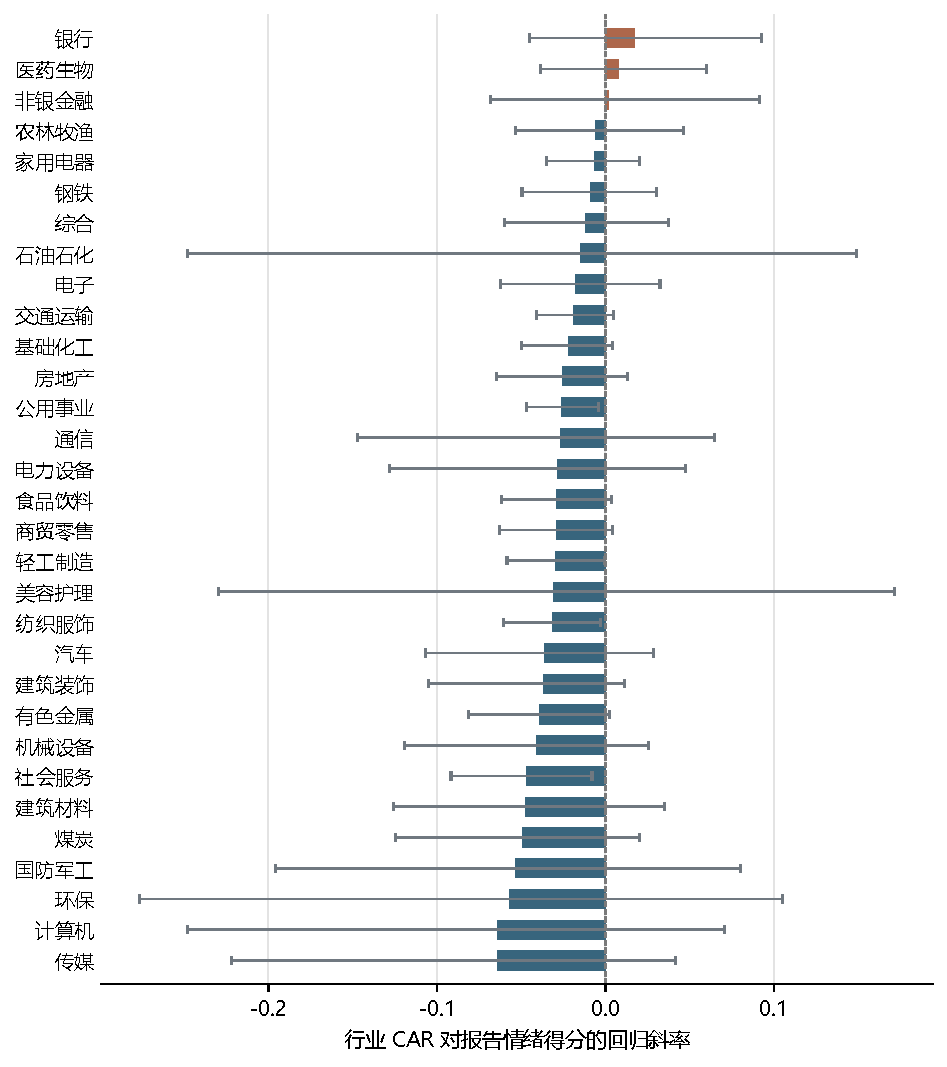
\includegraphics[width=0.96\linewidth,height=0.65\textheight,keepaspectratio]{fig19_heterogeneity.pdf}
  \caption{行业情绪敏感度与 95\% 置信区间（E5，按原始结果重排版）}\label{fig:industry-sensitivity}
\end{figure}

分析使用三项行业特征。利率敏感度由行业日超额收益对 10 年期国债收益率日变动的斜率度量，融资敏感度由行业月收益对社会融资规模累计同比变动的斜率度量。政策依赖指标将农林牧渔、银行、房地产、公用事业、建筑材料、建筑装饰及国防军工事先标为政策依赖行业。前两项在不同频率和覆盖长度下估计，第三项为定性代理。以行业估计斜率为因变量，在 31 个行业的横截面联合加入三项特征并使用 HC3 标准误，三项的原始 $p$ 值分别为 0.423、0.617 和 0.657。利率和融资敏感度分别单独入模时均达到 5\% 水平，但两者相关系数为 $-0.815$，联合估计难以区分相应关系。事件层面板另以 CAR 为因变量，保留行业固定效应并按事件聚类，逐一加入情绪与行业特征的交互项，三项的 $p$ 值均高于 0.10。

以 2014 年 2 月 21 日为界比较前后子样本，行业斜率的 Spearman 秩相关为 0.035（$p=0.897$），符号一致率为 38.7\%。由此，行业斜率存在数值差别，但联合横截面和事件层交互未为预设的三类特征提供稳定解释，跨时期的敏感行业排序也未复现。当前结果暂不支持 H3。

\subsection{大语言模型情绪及其增量}

E6 用大语言模型（LLM）对报告全文评分。固定模型别名 \texttt{qwen3.8-27b}、提示词 v1 和温度 0.0。分数取值 $[-1,1]$，综合政策立场、经济判断、风险、流动性和政策展望。提示词要求同时以结构化字段输出政策立场、各维度分数和原文依据，预测模型仅使用综合分数。103 期均得到可解析得分，其中部分报告在调整输出上限后获得有效响应。LLM 与 NTUSD 简体、DLUT、领域词典的 Pearson 相关分别为 0.213、0.326 和 0.042，说明评分差异需要结合下游结果和人工参照判断。

E6 沿用 E4 的面板、时间划分和信息集，用 LLM 分数与其滚动行业暴露构造交互项，比较词典模型、LLM 模型以及包含两个交互项的联合模型。测试期 LLM 的平均 IC 为 0.0733，词典为 $-0.0169$。LLM 的 IC 水平对零检验 $p=0.266$，与词典 IC 的点差不提供模型间显著改善的证据。LLM 的 $R^2_{\mathrm{OOS}}$ 低于词典，MAE 更大，验证期的排序指标也未同步改善。联合模型中 LLM 交互系数为 $-0.0272$（NW $p=0.684$），联合模型测试误差仍高于单独的 NTUSD 简体模型。评分差别与排序改善均不足以支持 H4 所要求的增量预测证据。

\subsection{多空组合及因子回归}

E7 把 E4 的样本外行业预测仅用作排序，持有期改为报告发布后的第一个完整自然季度。共形成 2016Q2 至 2026Q3 的 42 个组合季度，报告发布领先季初 35 至 57 个日历日。季初等权做多预测值最高的 5 个行业，等权做空最低的 5 个行业。多头和空头的绝对权重各为 100\%，按权重绝对变动的交易名义额计入单边 10 个基点的交易成本。无文本组合采用相同的行业池和持有期，另外保留同池行业等权、沪深 300 与随机分组用于参照。排序仍来自旧目标训练的模型，而且行业池沿用事后满足数据完整性要求的样本，组合结果用于描述排序在后移窗口内的表现。

图~\ref{fig:portfolio-equity}展示组合累计净值。计成本后，情绪多空组合的年化收益为 $-4.61\%$，夏普比率为 $-0.24$，最大回撤为 $-57.83\%$。无文本多空年化收益为 $-7.36\%$。分阶段看，情绪多空由验证期年化 $2.10\%$ 转为测试期 $-9.82\%$，测试期无文本为 $-8.59\%$。现有脚本以组合收益减去季度无风险收益为因变量，以中国三因子 CH3\cite{liuStambaughYuan2019}为自变量进行回归。因子覆盖不足的 2026Q2 和 2026Q3 从回归中剔除，保留 40 季。其截距季值经复利换算为年化 $2.65\%$（NW 滞后 1 阶，$t=0.46$）。该减无风险收益的约定与直接回归零成本多空价差的常见口径有别，不将其解释为标准零成本组合 alpha。收益仅反映设定的固定成本，组合实施还受融券供给、行业指数工具和市场冲击约束。

\paperfigure{fig18_portfolio_equity.pdf}{发布后完整季度的行业多空组合净值（E7，净成本与同池基准）}{fig:portfolio-equity}{0.96}

\subsection{模型结果小结}

回溯比较中，主词典模型在排序和误差指标上给出不同方向的变化。LLM 模型只提供局部排序改善，联合模型缺少显著增量。行业敏感度的排序和对行业特征的解释均缺乏跨设定支持。将组合收益移至发布后完整季度后，测试期也未观察到稳定的配置收益。下一章考察估计窗、文本来源及训练时点对这些结论的影响。

\section{进一步分析}\label{sec:further}

\subsection{事件窗、模型设定与多重检验}

E8 在事件模型和季度预测中改变词典、基准指数、窗口长度、样本切点、情绪编码、特征滞后及缩尾规则。49 个设定中，事件设定 23 个，旧收益窗口和时点修正窗口的预测设定各 13 个。39 个达到计算和最低样本要求，10 个在分组样本量、模型矩阵秩或固定测试期覆盖方面受限。事件对照按同一发行期与行业的交集比较，并在事件内等权汇总 CAR。季度预测对照在共同面板内重估，并按共同预测键计分。因此，使用中证全指后样本起点后移造成的差异，与同样本基准变化引起的差异分别记录。

事件比较用 $[0,+5]$ 作展示锚点，其他三个窗口同时列入检验。市场模型中，主词典的四个窗口下高减低 CAR 点估计同为负。$[0,+1]$ 的差为 $-0.609$ 个百分点（原始 $p=0.0113$），校正后的 $p$ 值为 0.2605。改用均值调整模型时，展示窗高减低差值转为正，原始 $p=0.485$。从估计窗中剔除与历史报告 $[0,+10]$ 窗口重叠的交易日后，差值为 $-0.574$ 个百分点（$p=0.247$）。这项处理针对估计窗重叠，同期市场消息仍有可能混入报告发布附近的收益。

事件主效应、旧口径预测系数、严格时点预测系数分别形成三个检验族，以 Benjamini--Hochberg（BH）与 Holm 法报告调整后的 $p$ 值\cite{benjaminiHochberg1995,holm1979}。原始 $p<0.05$ 的主效应共 3 项，两种调整后均无一项达到 5\% 水平。全样本平均 CAR 另列为次要检验族。不同设定重复使用相同报告与行业，BH 结果按探索性指标解释，Holm 提供对检验依赖结构要求较弱的校正。全部稳健性设定共记录 19,876 条底层失败或受限条目，其中部分条目对应多个行业或同一观测的不同设定。其数目不能解释为独立样本量。

\subsection{严格时点下的预测复核}\label{sec:strict-timing}

E8 将预测目标改为发布后的首个完整季度，并重估文本模型和无文本模型。模型以报告发布日期为预测原点，只用在该日期前已结束的历史收益季度更新系数，至少需 8 个可用历史拟合季度。旧口径的 2,274 个行业与季度观测均含发布前收益。修正后获得 2,243 个基础观测和 101 期报告，旧口径最后纳入的 2026Q2 报告对应的发布后完整季度落在观察期外。严格设定的预测记录均通过发布日及标签实现时点约束检查。已归档行情的行业分类、覆盖和事后补齐规则仍限制严格时点样本的解释。

\begin{table}[htbp]
  \centering\small
  \caption{发布后首个完整季度的配对测试结果（E8）}\label{tab:strict-oos}
  \begin{tabular}{lrrrr}
    \toprule
    模型 & 观测数 & 平均 IC & $R^2_{\mathrm{OOS}}$ & MAE \\
    \midrule
    无文本 & 674 & 0.0401 & $-0.5628$ & 0.08605 \\
    NTUSD 简体 & 674 & $-0.0074$ & $-0.9039$ & 0.09567 \\
    文本模型减无文本模型 & & $-0.0475$ & $-0.3410$ & 0.00962 \\
    \bottomrule
  \end{tabular}
  \par\smallskip
  \parbox{0.88\linewidth}{\footnotesize 注：两模型在共同面板上拟合，测试期均为 2021Q1 至 2026Q3，共 23 季。来源为 E8 严格时点参考设定的配对统计。}
\end{table}

严格时点结果见表~\ref{tab:strict-oos}。主词典在平均 IC、$R^2_{\mathrm{OOS}}$ 与 MAE 上均弱于无文本参照，交互系数均值为 $-0.0330$（NW 原始 $p=0.184$）。旧窗口下，NTUSD 简体与 DLUT 等权组合的个别样本外指标相对无文本模型略有改善，时点修正后该组合的增量 $R^2_{\mathrm{OOS}}$ 转为负。两套评估共同表明 H2 缺少稳定支持，其中严格时点口径只评价词典特征。LLM 特征仍需按同样的时点要求另行验证。

\subsection{LLM 敏感性与失败归因}

E9 冻结原始响应，在同一批 E6 响应上重放严格解析、E6 宽松解析及括号规范化三种审计规则，103 期均得到一致得分。配置比较使用新版逐响应审计与汇总表。按 E6 宽松解析，同一较早提示词在温度 0.0 下取得 91 期有效分数，提高至 0.7 后只有 31 期有效。高温设置的 67 次请求受 HTTP 429 限流，返回的 36 份中另有 5 份在输出触顶后未通过 JSON 解析。最简提示词在温度 0.7 的 103 次请求全部受限流，缺少可用于归因的模型响应。仅比较同一提示词在两种温度下共同有效的响应时，旧版提示词的分数 Pearson 相关约为 0.988。现有记录能量化输出可用性，温度对分数的独立作用还受共同样本选择影响。

跨模型比较原计划覆盖 39 期，归档请求清单每种别名覆盖 24 期。\texttt{gpt-4o} 的 24 期均可用，但可计算模型指标的验证期只有 2 季（平均 IC 为 0.322），测试期也只有 6 季（$-0.0374$）。\texttt{deepseek-v4-flash} 有效输出 17 期，\texttt{glm-5.3} 的请求全部受限流。模型比较样本稀疏，模型别名未绑定可核实的权重版本，且预测口径沿用 E6 的回溯窗口。这些条件限制了对提示词、模型和温度的横向比较。

\subsection{误差、异常与推断边界}

E10 对冻结输入作只读检查，记录 1,002 条复核条目。其中，521 条为市场交易日缺失或行情覆盖限制，287 条为预测残差异常，33 条为低词典覆盖抽检，29 条为 LLM 变体失败。异常残差按绝对值超过四分位距上栅栏判定。E8 严格时点的文本和无文本预测中，共有 57 条残差异常（1,348 条模型预测记录），异常组与其余组的平均绝对残差分别为 0.3274 和 0.0804。不同模型可能在同一行业季度同时出现异常，数量用于定位误差来源。另有 15 条人工评分待办来自 E10 生成时的快照。其后评分表已填入分数，评分人身份与独立重复评分的证据仍待补齐。

本文所用的解释变量来自季度报告中的共同信息，时间维度的有效观察数远少于行业与季度面板的行数。报告文字可能在同一文本中同时表达当前经济风险和未来宽松意图，单一情绪得分难以区分两者。行业敏感度还受行业历史覆盖、代理变量共线性、极端收益和正常收益模型选择制约。事件日后短窗与严格季度预测回答不同时间尺度的问题。现有证据在两种时间尺度上均不足以支撑稳定的正向收益关系，但仍容许不同文本维度、不同政策背景或不同观察频率下存在更局部的关系。

\FloatBarrier
\section{结论与启示}\label{sec:conclusion}

\subsection{研究结论}
本研究从报告发布、行业收益的实现时间以及训练样本的可用时间出发，检验货币政策文本情绪能否用于 A 股行业收益预测。按本稿的暂定阈值，H1 仅获初步、部分支持。NTUSD 与归档抽检分值的 Pearson 相关为 $0.695$，与 DLUT 的相关为 $0.829$。抽检分值的来源和独立性仍待核验，不能将数值条件满足直接视作独立人工效度验证。

H2 未获支持。主事件窗及不同设定中出现的未校正显著性经多重检验校正后消失。以报告期的下一季度定义收益时，主词典模型在共同样本上的样本外 $R^2$ 低于无文本基准。按发布后第一个完整季度定义收益并约束训练时点后，差距仍为负（$\Delta R^2=-0.341$）。H3 暂未获支持。三类行业特征代理在联合截面回归中均未达预设显著性水平，前后子样本行业敏感度排序接近不相关。H4 未获支持。基准提示词下，大语言模型的平均秩相关有所提高，但点预测误差扩大，其联合模型系数也缺乏统计支持。

\subsection{与已有文献的对话}
姜富伟等将货币政策报告文本与市场层面的资产价格联系起来\cite{jiangHuHuang2021}。对全市场共同成分有解释力的季度信号，只有在行业暴露存在稳定差异时才可能改善截面排序。本文对行业敏感度的检验与林雨欣研究央行沟通行业差异的方向相近\cite{linYuxin2025}，联合代理检验与跨期稳定性检验为比较提供了可复核的量化依据。国外研究分别从政策沟通的措辞及货币政策目标推断入手\cite{luccaTrebbi2009,shapiroWilson2022}。沟通载体、制度背景、估计对象和收益频率的差异限制了跨研究比较。本稿的贡献在于以相同报告集比较两类度量方式，并识别收益窗口和可用信息约束对于评判行业预测力的重要性。

\subsection{实践启示、局限与展望}
现有结果不支持将单一文本情绪分数直接用于行业轮动。研究设计可以进一步区分回顾性经济判断与前瞻性政策指引，比较措辞变化、可读性与政策主题等特征，并将跨期验证和收益实现约束写入实验协议。更细的发布时点和交易频率有助于缩短事件窗，独立双人评分及复评可检验报告情绪的测量误差。正则化或树模型需要在相同信息集和共同测试样本上重新评估。

本研究的有效时间单位主要是季度。历史估计窗重叠、部分事件窗中同期政策公告、行业行情起点差异，以及宏观数据未完全实现历史版本控制，均会影响估计或复现。少量报告的抽检评分缺乏完整的来源和复评记录。大语言模型调用的底层修订号亦不可得。以上证据主要用于关联描述与预测评价，适用范围限于现有样本、收益频率和模型。

\subsection{数据与代码可用性}
实验脚本、运行日志、输入清单及图表对应关系见附录\ref{sec:reproduction}。报告原文可由人民银行公开栏目与项目索引定位。完整报告缓存、宏观与利率缓存、外部因子文件和原始模型响应按来源许可与项目记录管理。初稿以行业汇总行情和公开政策文本为核心实证材料。署名贡献、资助及利益冲突事项由团队于定稿时核定。人机分工详见赛事单独提交的声明。

\FloatBarrier
\clearpage
\printbibliography[heading=bibintoc,title={参考文献}]
\clearpage
\FloatBarrier
\appendix
\ctexset{section={name={附录\ ,},number=\Alph{section}}}
\renewcommand{\thesection}{\Alph{section}}
\section{数据、代码与结果追溯}\label{sec:reproduction}

表\ref{tab:provenance}列出实验产物与论文证据的对应关系。路径以项目根目录为起点。

\begin{table}[!htbp]
\centering\small
\caption{主要结论的核验材料}\label{tab:provenance}
\begin{tabularx}{\linewidth}{@{}l>{\raggedright\arraybackslash}X@{}}
\toprule
证据 & 核验材料 \\
\midrule
报告索引与文本度量 & \path{experiments/E1/mpr_index_full.csv} 记录发布日期、原文链接和 SHA-256。\path{experiments/E1/validation/} 保留词典及抽检对照。\\
事件研究 & \path{experiments/E2/} 与 \path{experiments/E3/} 留存事件窗结果、估计模型、分组汇总及异常记录。\\
收益预测与行业异质性 & \path{experiments/E4/e4_oos_metrics.csv}、\path{experiments/E5/e5_cross_section.csv} 和 \path{experiments/E5/e5_stability.csv} 记录预测指标、行业特征的截面估计及跨期稳定性。\\
大语言模型与组合 & \path{experiments/E6/e6_llm_oos_metrics.csv} 与 \path{experiments/E6/e6_llm_incremental_regression.csv} 对应模型比较。\path{experiments/E7/e7_metrics.json} 对应组合和因子回归。\\
稳健性与时点核验 & \path{experiments/E8/e8_robustness_summary.csv} 记录时点修正和多重检验。\path{experiments/E8/e8_input_manifest.csv} 记录冻结输入。\\
敏感性与错误审计 & \path{experiments/E9/e9_response_audit.csv} 与 \path{experiments/E9/e9_prompt_model_manifest.json} 登记模型响应与调用配置。\path{experiments/E10/e10_anomaly_samples.csv} 保留异常快照。\\
\bottomrule
\end{tabularx}
\end{table}

完整报告文本可按 E1 索引重取，项目保留 E0 的五期样本供检查。指数行情获取方式与缺失记录见《数据来源说明》。接口软件的开源许可与上游行情、词典及政策文本的再分发权限分别适用。原始模型响应、宏观与利率缓存及外部因子镜像位于本地缓存。跨环境复现需要重新获取相应输入并对照冻结清单和哈希。采用同名模型重新调用时，评分可能随服务端修订而变化。

图表由项目的图表目录下的绘图脚本生成。实验图表输入可由 \path{build_experiment_inputs.py} 从既有输出汇总。正文对比指标优先使用各实验明确标记的共同样本。复算时应同时核对收益窗口、截面基准及拟合时点。

\end{document}
